% ==== Document Class & Packages =====
\documentclass[12pt,hidelinks]{article}
\usepackage[explicit]{titlesec}
\usepackage{titletoc}
\usepackage{tocloft}
\usepackage{charter}
\usepackage[many]{tcolorbox}
\usepackage{amsmath}
\usepackage{graphicx}
\usepackage{xcolor}
\usepackage{tikz,lipsum,lmodern}
\usetikzlibrary{calc}
\usepackage[spanish, mexico]{babel}
\usepackage{fancyhdr}
\usepackage{mathrsfs}
\usepackage{empheq}
\usepackage{fourier}% change to lmodern if fourier is no available
\usepackage{wrapfig}
\usepackage{fancyref}
\usepackage{hyperref}
\usepackage{cleveref}
\usepackage{listings}
\usepackage{varwidth}
\usepackage{longfbox}
\usepackage{geometry}
\usepackage{marginnote}
\usepackage[utf8]{inputenc}
\tcbuselibrary{theorems}
\tcbuselibrary{breakable, skins}
\tcbuselibrary{listings, documentation}
\geometry{
	a4paper,
	left=33mm,
	right=33mm,
	top=20mm}
% ========= Path to images ============
%   - Direct the computer on the path 
% 	  to the folder containg the images
% =====================================
\graphicspath{{./images/}}
% ============= Macros ================
\newcommand{\fillin}{\underline{\hspace{.75in}}{\;}}
\newcommand{\solution}{\textcolor{mordantred19}{Solution:}}
\setlength{\parindent}{0pt}
\addto{\captionsenglish}{\renewcommand*{\contentsname}{Table of Contents}}
\linespread{1.2}
% ======== Footers & Headers ==========
\cfoot{\thepage}
\chead{}\rhead{}\lhead{}
% =====================================
\renewcommand{\thesection}{\arabic{section}}
\newcommand\sectionnumfont{% font specification for the number
	\fontsize{380}{130}\color{myblueii}\selectfont}
\newcommand\sectionnamefont{% font specification for the name "PART"
	\normalfont\color{white}\scshape\small\bfseries }
% ============= Colors ================
% ----- Red -----
\definecolor{mordantred19}{rgb}{0.68, 0.05, 0.0}
% ----- Blue -----
\definecolor{st.patrick\'sblue}{rgb}{0.14, 0.16, 0.48}
\definecolor{teal}{rgb}{0.0, 0.5, 0.5}
\definecolor{beaublue}{rgb}{0.74, 0.83, 0.9}
\definecolor{mybluei}{RGB}{0,173,239}
\definecolor{myblueii}{RGB}{63,200,244}
\definecolor{myblueiii}{RGB}{199,234,253}
% ---- Yellow ----
\definecolor{blond}{rgb}{0.98, 0.94, 0.75}
\definecolor{cream}{rgb}{1.0, 0.99, 0.82}
% ----- Green ------
\definecolor{emerald}{rgb}{0.31, 0.78, 0.47}
\definecolor{darkspringgreen}{rgb}{0.09, 0.45, 0.27}
% ---- White -----
\definecolor{ghostwhite}{rgb}{0.97, 0.97, 1.0}
\definecolor{splashedwhite}{rgb}{1.0, 0.99, 1.0}
% ---- Grey -----
\definecolor{whitesmoke}{rgb}{0.96, 0.96, 0.96}
\definecolor{lightgray}{rgb}{0.92, 0.92, 0.92}
\definecolor{floralwhite}{rgb}{1.0, 0.98, 0.94}
% ========= Part Format ==========
\titleformat{\section}
{\normalfont\huge\filleft}
{}
{20pt}
{\begin{tikzpicture}[remember picture,overlay]
	\fill[myblueiii] 
	(current page.north west) rectangle ([yshift=-13cm]current page.north east);   
	\node[
	fill=mybluei,
	text width=2\paperwidth,
	rounded corners=6cm,
	text depth=18cm,
	anchor=center,
	inner sep=0pt] at (current page.north east) (parttop)
	{\thepart};%
	\node[
	anchor=south east,
	inner sep=0pt,
	outer sep=0pt] (partnum) at ([xshift=-20pt]parttop.south) 
	{\sectionnumfont\thesection};
	\node[
	anchor=south,
	inner sep=0pt] (partname) at ([yshift=2pt]partnum.south)   
	{\sectionnamefont SECTION};
	\node[
	anchor=north east,
	align=right,
	inner xsep=0pt] at ([yshift=-0.5cm]partname.east|-partnum.south) 
	{\parbox{.7\textwidth}{\raggedleft#1}};
	\end{tikzpicture}%
}
% ========= Hyper Ref ===========
\hypersetup{
	colorlinks,
	linkcolor={red!50!black},
	citecolor={blue!50!black},
	urlcolor={blue!80!black}
}
% ========= Example Boxes =============
\tcbset{
	defstyle/.style={
		fonttitle=\bfseries\upshape, 
		fontupper=\slshape,
		arc=0mm, 
		beamer,
		colback=blue!5!white,
		colframe=blue!75!black},
	theostyle/.style={
		fonttitle=\bfseries\upshape, 
		fontupper=\slshape,
		colback=red!10!white,
		colframe=red!75!black},
	visualstyle/.style={
		height=6.5cm,
		breakable,
		enhanced,
		leftrule=0pt,
		rightrule=0pt,
		bottomrule=0pt,
		outer arc=0pt,
		arc=0pt,
		colframe=mordantred19,
		colback=lightgray,
		attach boxed title to top left,
		boxed title style={
			colback=mordantred19,
			outer arc=0pt,
			arc=0pt,
			top=3pt,
			bottom=3pt,
		},
		fonttitle=\sffamily,},
	discussionstyle/.style={
		height=6.5cm,
		breakable,
		enhanced,
		rightrule=0pt,
		toprule=0pt,
		outer arc=0pt,
		arc=0pt,
		colframe=mordantred19,
		colback=lightgray,
		attach boxed title to top left,
		boxed title style={
			colback=mordantred19,
			outer arc=0pt,
			arc=0pt,
			top=3pt,
			bottom=3pt,
		},
		fonttitle=\sffamily},
	mystyle/.style={
		height=6.5cm,
		breakable,
		enhanced,
		rightrule=0pt,
		leftrule=0pt,
		bottomrule=0pt,
		outer arc=0pt,
		arc=0pt,
		colframe=mordantred19,
		colback=lightgray,
		attach boxed title to top left,
		boxed title style={
			colback=mordantred19,
			outer arc=0pt,
			arc=0pt,
			top=3pt,
			bottom=3pt,
		},
		fonttitle=\sffamily},
	aastyle/.style={
		height=3.5cm,
		enhanced,
		colframe=teal,
		colback=lightgray,
		colbacktitle=floralwhite,
		fonttitle=\bfseries,
		coltitle=black,
		attach boxed title to top center={
			yshift=-0.25mm-\tcboxedtitleheight/2,
			yshifttext=2mm-\tcboxedtitleheight/2}, 
		boxed title style={boxrule=0.5mm,
			frame code={ \path[tcb fill frame] ([xshift=-4mm]frame.west)
				-- (frame.north west) -- (frame.north east) -- ([xshift=4mm]frame.east)
				-- (frame.south east) -- (frame.south west) -- cycle; },
			interior code={ 
				\path[tcb fill interior] ([xshift=-2mm]interior.west)
				-- (interior.north west) -- (interior.north east)
				-- ([xshift=2mm]interior.east) -- (interior.south east) -- (interior.south west)
				-- cycle;} }
	},
	examstyle/.style={
		height=9.5cm,
		breakable,
		enhanced,
		rightrule=0pt,
		leftrule=0pt,
		bottomrule=0pt,
		outer arc=0pt,
		arc=0pt,
		colframe=mordantred19,
		colback=lightgray,
		attach boxed title to top left,
		boxed title style={
			colback=mordantred19,
			outer arc=0pt,
			arc=0pt,
			top=3pt,
			bottom=3pt,
		},
		fonttitle=\sffamily},
	doc head command={
		interior style={
			fill,
			left color=yellow!20!white, 
			right color=white}},
	doc head environment={
		boxsep=4pt,
		arc=2pt,
		colback=yellow!30!white,
	},
	doclang/environment content=text
}
% ============= Boxes ================
\newtcolorbox[auto counter,number within=section]{example}[1][]{
	mystyle,
	title=Example~\thetcbcounter,
	overlay unbroken and first={
		\path
		let
		\p1=(title.north east),
		\p2=(frame.north east)
		in
		node[anchor=
		west,
		font=\sffamily,
		color=st.patrick\'sblue,
		text width=\x2-\x1] 
		at (title.east) {#1};
	}
}
\newtcolorbox[auto counter,number within=section]{longexample}[1][]{
	examstyle,
	title=Example~\thetcbcounter,
	overlay unbroken and first={
		\path
		let
		\p1=(title.north east),
		\p2=(frame.north east)
		in
		node[anchor=
		west,
		font=\sffamily,
		color=st.patrick\'sblue,
		text width=\x2-\x1] 
		at (title.east) {#1};
	}
}
\newtcolorbox[auto counter,number within=section]{example2}[1][]{
	aastyle,
	title=Example~\thetcbcounter,{}
}
\newtcolorbox[auto counter,number within=section]{discussion}[1][]{
	discussionstyle,
	title=Discussion~\thetcbcounter,
	overlay unbroken and first={
		\path
		let
		\p1=(title.north east),
		\p2=(frame.north east)
		in
		node[anchor=
		west,
		font=\sffamily,
		color=st.patrick\'sblue,
		text width=\x2-\x1] 
		at (title.east) {#1};
	}
}
\newtcolorbox[auto counter,number within=section]{visualization}[1][]{
	visualstyle,
	title=Visualization~\thetcbcounter,
	overlay unbroken and first={
		\path
		let
		\p1=(title.north east),
		\p2=(frame.north east)
		in
		node[anchor=
		west,
		font=\sffamily,
		color=st.patrick\'sblue,
		text width=\x2-\x1] 
		at (title.east) {#1};
	}
}
% --------- Theorems ---------
\newtcbtheorem[number within=subsection,crefname={definition}{definitions}]%
{Definition}{Definition}{defstyle}{def}%
\newtcbtheorem[use counter from=Definition,crefname={theorem}{theorems}]%
{Theorem}{Theorem}{theostyle}{theo}
%
\newtcbtheorem[use counter from=Definition]{theo}{Theorem}%
{
	theorem style=plain,
	enhanced,
	colframe=blue!50!black,
	colback=yellow!20!white,
	coltitle=red!50!black,
	fonttitle=\upshape\bfseries,
	fontupper=\itshape,
	drop fuzzy shadow=blue!50!black!50!white,
	boxrule=0.4pt}{theo}
\newtcbtheorem[use counter from=Definition]{DashedDefinition}{Definition}%
{
	enhanced,
	frame empty,
	interior empty,
	colframe=darkspringgreen!50!white,
	coltitle=darkspringgreen!50!black,
	fonttitle=\bfseries,
	colbacktitle=darkspringgreen!15!white,
	borderline={0.5mm}{0mm}{darkspringgreen!15!white},
	borderline={0.5mm}{0mm}{darkspringgreen!50!white,dashed},
	attach boxed title to top center={yshift=-2mm},
	boxed title style={boxrule=0.4pt},
	varwidth boxed title}{theo}
%%%%%%%%%%%%%%%%%%%%%%%%%%%%%%%%%%%%%%%%
\newtcblisting[auto counter,number within=section]{disexam}{
	skin=bicolor,
	colback=white!30!beaublue,
	colbacklower=white,
	colframe=black,
	before skip=\medskipamount,
	after skip=\medskipamount,
	fontlower=\footnotesize,
	listing options={style=tcblatex,texcsstyle=*\color{red!70!black}},}
%%%%%%%%%%%%%%%%%%%%%%%%%%%%%%%%%%%%%%%

\begin{document}
	\begin{titlepage}
		\centering % Center everything on the title page
		\scshape % Use small caps for all text on the title page
		\vspace*{1.5\baselineskip} % White space at the top of the page
		% ===================
		%	Title Section 	
		% ===================
		
		\rule{13cm}{1.6pt}\vspace*{-\baselineskip}\vspace*{2pt} % Thick horizontal rule
		\rule{13cm}{0.4pt} % Thin horizontal rule
		
		\vspace{0.75\baselineskip} % Whitespace above the title
		% ========== Title ===============	
		{	\Huge Manual estadística y probabilidad con Python y R }
		% ======================================
		\vspace{0.75\baselineskip} % Whitespace below the title
		\rule{13cm}{0.4pt}\vspace*{-\baselineskip}\vspace{3.2pt} % Thin horizontal rule
		\rule{13cm}{1.6pt} % Thick horizontal rule
		
		\vspace{1.75\baselineskip} % Whitespace after the title block
		% =================
		%	Information	
		% =================
		{\large Realizado por:
			\vspace*{1.2\baselineskip}\\
			Glen Nicolás Rico\\
			Maykoll Gil\\
			Miguel Gómez
		}\\
		\vfill
		
	\end{titlepage}
	%%%%%%%%%%%%%%%%%%%%%%%%%%%%%%%%%%%%%%%%%%%%%%%%%%%%%%%%%%%
	\tableofcontents
	\vfill
	\small{\noindent \textbf{Acerca de éste documento} \vspace{-3mm}\\
		\noindent \rule{3.3cm}{0.5pt} \\
		Este documento fue creado para el beneficio de todos los estudiantes que desean utilizar R y Python para entender algunos conceptos de probabilidad y estadística.}
	\newpage
	\newgeometry{
		left=29mm, 
		right=29mm, 
		top=20mm, 
		bottom=15mm}
	%%%%%%%%%%%%%%%%%%%%%%%%%%%%%%%%%%%%%%%%%%%%%%%%%%%%%%%%%%%
	\section{Breve introducción a R y Python}
	\vspace{10.5cm}
	En esta sección vamos a preparar el entorno con el que se van a ejecutar todos los ejemplos presentados en este libro, por lo que si ya tiene alguna instalación de R y Python sólo resta verificar la versión, a fecha de este documento las versiones estables que utilizaremos son:
	\begin{itemize}
		\item R 3.5.3
		\item R-studio 1.2.5019
		\item Python 3.8.
	\end{itemize}
	en este manual no vamos a profundizar en el lenguaje, por lo que una versión compatible con python 3 es suficiente para los ejemplos que vamos a ver aquí.
	\subsection{Descarga e instalación de R y R-Studio}
	R es un lenguaje y entorno de de código libre bajo la licencia GNU y R Studio no esde código abierto pero es una herramienta muy útil para el manejo de R, y es por ello que lo instalaremos. Estos son los links de descarga
	\begin{itemize}
		\item Para descargar únicamente R ir a\url{https://www.r-project.org/}, allí se encuentran los enlaces de descarga de R, se recomienda descargar la versión más estable si hasta ahora se está iniciando en R.
		\item Si se quiere llevar a cabo una instalación completa junto con R, R-studio es la mejor opción, para descargarlo ir a \url{https://rstudio.com/} allí se encuentra el link que redirige a la versión Free. Usualmente ocurre que se debe elegir la versión de R que se va instalar dependiendo del sistema operativo, en este manual, sin embargo si lleva tiempo utilizando cualquier sistema operativo encontrará bastante sencilla su instalación.
	\end{itemize}
	\textit{Nota:} La única versión que no se recomienda descargar en cualquier caso es la descarga del código fuente, si la descarga deberá compilar el código desde cero (\textit{from scratch}), es mucho más complicado, sólo se recomienda para usuarios avanzados.	
	\subsubsection{Instalación de R (Si no desea instalar r-studio)}
	La instalación es muy sencilla, primero ejecute el .exe descargado en la página de R.
	\begin{center}
		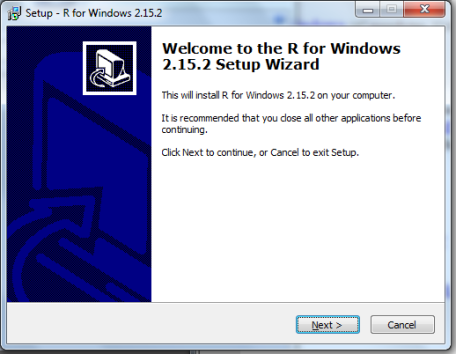
\includegraphics[scale=0.9]{images/1/install3-1.png}
	\end{center}
	Al dar siguiente estamos aceptando los términos de uso de la licencia GNU
	\begin{center}
		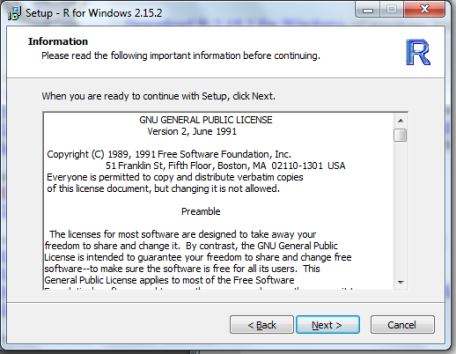
\includegraphics[scale=0.9]{images/1/install3-2.png}
	\end{center}
	, dependiendo de la arquitectura de su computador deberá elegir entre un tipo de instalación, usualmente el valor por defecto del instalador tiene la elección que requiere
	\begin{center}
		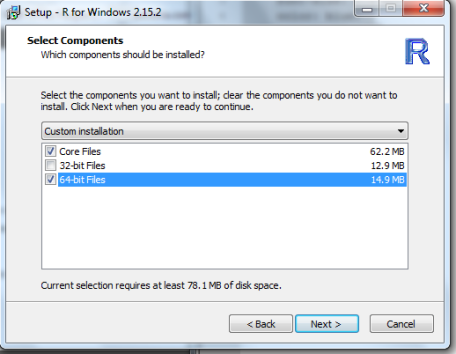
\includegraphics[scale=0.9]{images/1/install3-3.png}
	\end{center}
	En los siquientes pasos daremos siguiente, eventualmente llegaremos a
	\begin{center}
		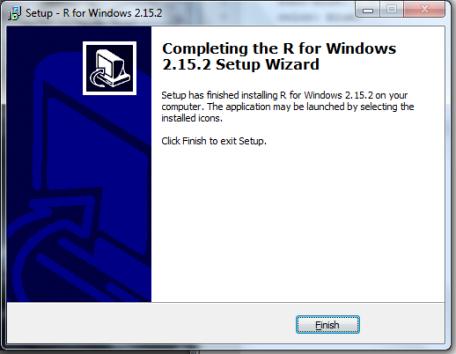
\includegraphics[scale=0.9]{images/1/install3-4.png}
	\end{center}
	Al finalizar, ya tendremos instalado R.
	\subsubsection{Instalación de R-studio}
	La instalación es muy sencilla, primero ejecute el .exe descargado en la página de R.
	\begin{center}
		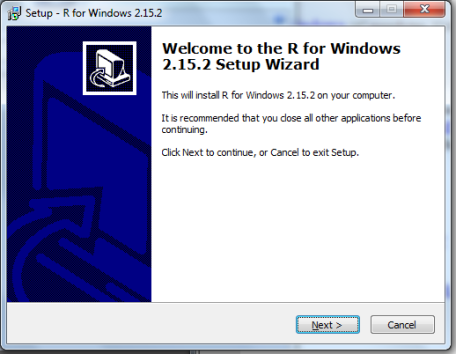
\includegraphics[scale=0.9]{images/1/install3-1.png}
	\end{center}
	Al dar siguiente estamos aceptando los términos de uso de la licencia GNU
	\begin{center}
		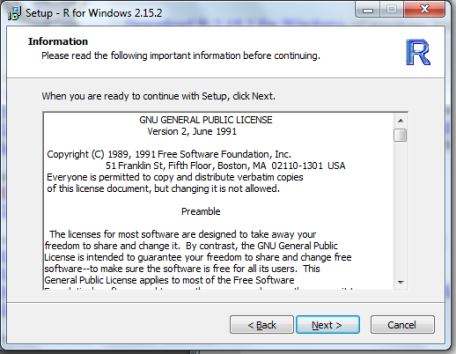
\includegraphics[scale=0.9]{images/1/install3-2.png}
	\end{center}
	, dependiendo de la arquitectura de su computador deberá elegir entre un tipo de instalación, usualmente el valor por defecto del instalador tiene la elección que requiere
	\begin{center}
		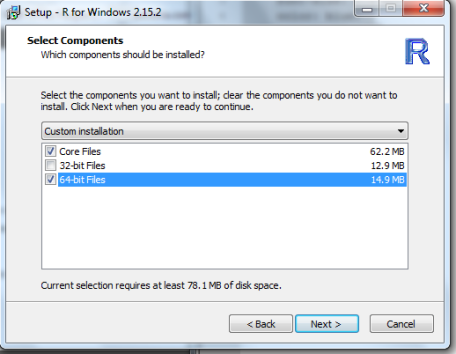
\includegraphics[scale=0.9]{images/1/install3-3.png}
	\end{center}
	En los siquientes pasos daremos siguiente, eventualmente llegaremos a
	\begin{center}
		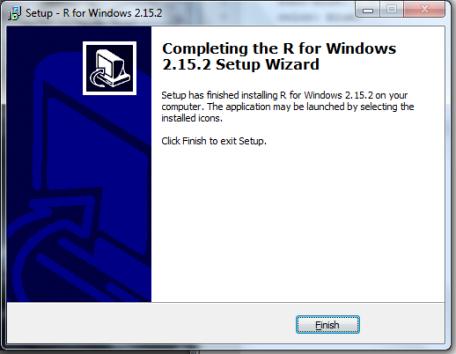
\includegraphics[scale=0.9]{images/1/install3-4.png}
	\end{center}
	Al finalizar, ya tendremos instalado R.
	\subsection{Descarga de Python}
	La instalación es muy sencilla, primero ejecute el .exe descargado en la página de R.
	\begin{center}
		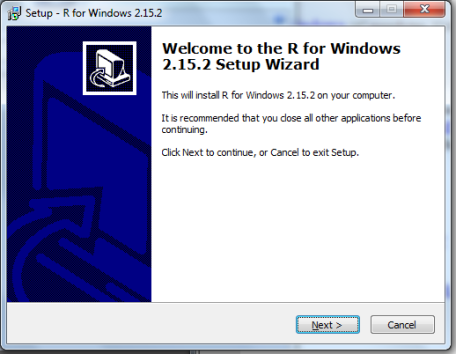
\includegraphics[scale=0.9]{images/1/install3-1.png}
	\end{center}
	Al dar siguiente estamos aceptando los términos de uso de la licencia GNU
	\begin{center}
		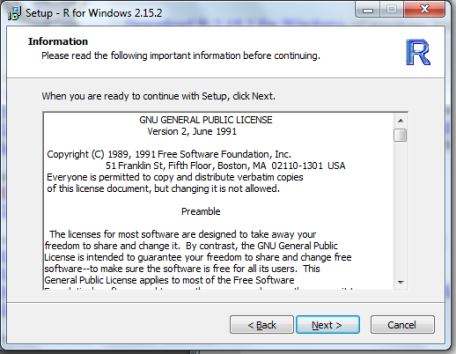
\includegraphics[scale=0.9]{images/1/install3-2.png}
	\end{center}
	, dependiendo de la arquitectura de su computador deberá elegir entre un tipo de instalación, usualmente el valor por defecto del instalador tiene la elección que requiere
	\begin{center}
		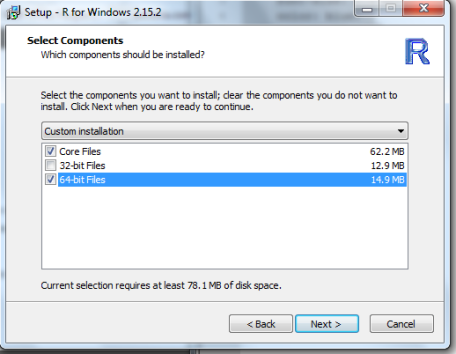
\includegraphics[scale=0.9]{images/1/install3-3.png}
	\end{center}
	En los siquientes pasos daremos siguiente, eventualmente llegaremos a
	\begin{center}
		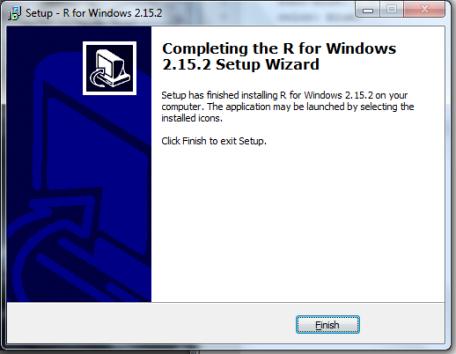
\includegraphics[scale=0.9]{images/1/install3-4.png}
	\end{center}
	Al finalizar, ya tendremos instalado R.
	\subsection{Código Fuente de los ejemplos presentados en el manual}
	Los fuentes de la construcción de este libro así como los ejemplos se encuentran en LINK DE GITHUB.
	\subsection{El lenguaje R}
	El lenguaje R es un lenguaje y entorno para el desarrollo de aplicaciones estadísticas, computacionales y gráficas.
	\paragraph{}R ofrece un amplio conjunto de herramientas estadísticas (para modelamiento, pruebas de hipótesis), herramientas gráficas y es altamente extensible, actualmente es uno de los proyectos de software libre más grandes del mundo, lo cual es una de sus fortalezas ya que al ser un proyecto de código abierto (en el que cualquiera puede aportar) toda la comunidad que utilza el software se beneficia de las contribuciones de todos, haciendo que R sea una herramienta en crecimiento y de uso extendido.
	\paragraph{} Este lenguaje tiene soporte para diferentes sistemas operativos.
	\subsubsection{El entorno}
	Cuando decimos que R también es un entorno, es debido a que no sólamente tiene las funciones que normalmente encontramos en un lenguaje de programación sino que también tiene un amplio abanico en crecimiento de 'paquetes'\footnote{Que son componentes adicionales que se pueden instalar según sea necesario.} para manipulación de texto, carga de archivos que a su vez pueden ser extendidas. R ha sido escrito deuna manera muy similar a los lenguajes de programación interpretados con el rendimiento del lenguaje de programación C.
	\subsubsection{Sintáxis}
	Como todo lenguaje debemos comprender algunas reglas básicas, a éstas reglas las conocemos como la sintáxis del lenguaje, dentro de esto encontramos varias categorías:
	\begin{itemize}
		\item \textbf{Definición y declaración de variables}. En todo lenguaje declaramos variables por lo que aprenderemos a definir variables junto con los tipos de datos en un programa R.
		\item \textbf{Operadores}. Repasaremos las operaciones básicas en R.
		\item \textbf{Estructuras de control}. Aquí ubicamos a las estructuras condicionales, condiciones en donde evaluamos el valor de verdad de una sentencia que permite alterar el flujo de un programa.
		\item  \textbf{Estructuras de repetición}. Aquí se encuentran las estructuras que nos permiten iterar, por ejemplo recorrer un archivo.
		\item \textbf{Funciones}. Son piezas de código, que nos ayudan a organizar el código. En general son una muy buena práctica de programación.
	\end{itemize}
	\subsubsection{Definición y declaración de variables}
	Primero repasaremos sobre los tipos de datos en R. R utiliza el paradigma de la orientación a objetos al límite, cada elemento en R es un objeto. R tiene $6$ tipos de datos:
	\begin{itemize}
		\item caracter. "a", "b", "hola"
		\item numérico. 2, 3, 3.14
		\item entero. 28L, 3L. el caracter L le indica a R que almacene el dato como un entero.
		\item lógico. TRUE, FALSE.
		\item complejo. 3+14i. En este manual no utilizaremos este tipo de datos para los problemas que manejamos es suficiente con los reales.
	\end{itemize}
	Ejemplo:
	\begin{verbatim}
		x <- "Hola"
		x
	\end{verbatim}
	Salida:
	\begin{verbatim}
		[1] "Hola"
	\end{verbatim}
	De esta forma acabamos de declarar una variable en R. Nótese que no fue necesario llevar a cabo una declaración del tipo de variable, R se encarga de asignar el tipo de dato dependiendo de lo que recibe. Por ejemplo:
	\begin{verbatim}
		x <- 1
		x
	\end{verbatim}
	Salida:
	\begin{verbatim}
		[1] 1
	\end{verbatim}
	
	Adicionalmente R también se encuentra provisto de funciones que nos permiten identificar propiedades de los objetos que declaramos:
	\begin{itemize}
		\item \texttt{class()}. Nos permite obtener la clase a la que está asociada a un objeto.
		\item \texttt{typeof()}. Nos permite obtener el tipo de dato de de una variable.
		\item \texttt{length()}. Nos permite obtener la longitud de un tipo de dato.
		\item \texttt{attributes()}. nos permite conocer si un objeto tiene determinados metadatos.
	\end{itemize}
	Ejemplo:
	\begin{verbatim}
		x <- 1L
		class(x)
		typeof(x)
		length(x)
		attributes(x)
	\end{verbatim}
	Salida:
	\begin{verbatim}
		class(x)
		[1] "integer"
		typeof(x)
		[1] "integer"
		length(x)
		[1] 1
		attributes(x)
		[1] NULL
	\end{verbatim}
	Cuando declaramos el tipo de dato sabíamos que era un entero, es por ello que obtenemos como tipo de dato y clase \texttt{integer}, como solo hemos ocupado 1 byte para almacenar el valor '1' obtenemos como valor de la función 1. Finalmente, \texttt{x} es un valor escalar, es por ello que no posee atributos y obtenemos el valor \texttt{NULL}, que indica que no tiene ningún atributo.
	\paragraph{} R cuenta con estructuras de datos para contener colecciones, nombraremos algunas de ellas:
	\begin{itemize}
		\item vectores atómicos.
		\item listas.
		\item matrices.
		\item data frame.
		\item factores.
	\end{itemize}
	En aplicaciones estadísticas encontraremos que es muy frecuente el uso de este tipo de estructuras.
	Los vectores se pueden declarar con varias funciones, las más comunes son \texttt{vector, logical, character, integer, numeric}.
	\paragraph{}Ejemplo:
	\begin{verbatim}
		vector()
		vector("character", length = 5)
	\end{verbatim}
	Salida
	\begin{verbatim}
		vector()
		[1] logical(0)
		vector("character", length = 5)
		[1] "" "" "" "" ""
	\end{verbatim}
	Con las funciones anteriores podemos analizar estos objetos.
	\paragraph{Matrices} las matrices son una extensión de los vectores pero tienen varias mas de una dimensión. Ejemplo:
	\begin{verbatim}
		m <- matrix(nrow = 2, ncol = 2)
		m
	\end{verbatim}
	Salida:
	\begin{verbatim}
			[,1]	[,2]
		[1,]	NA	NA
		[2,]	NA	NA
	\end{verbatim}
	\paragraph{Listas} Las listas en R actúan como contenedores. A diferencia de los vectores atómicos las listas puden contener diferentes tipos de datos, por ejemplo:
	\begin{verbatim}
		x <- list(1, "hola", TRUE, 3+14i)
		x	
	\end{verbatim}
	salida:
	\begin{verbatim}
		[[1]]
		[1] 1
		[[2]]
		[1] "hola"
		[[3]]
		[1] TRUE
		[[4]]
		[1] 3 + 14i
	\end{verbatim}
\end{document}